% CVPR 2024 Paper Template
% Accent-Robust ASR using Wav2Vec 2.0 with Adversarial Training

\documentclass[10pt,twocolumn,letterpaper]{article}

\usepackage{cvpr}
\usepackage{times}
\usepackage{epsfig}
\usepackage{graphicx}
\usepackage{amsmath}
\usepackage{amssymb}
\usepackage{booktabs}
\usepackage{multirow}
\usepackage{array}
\usepackage{microtype}
\usepackage{hyperref}
\usepackage{xcolor}
\usepackage{algorithm}
\usepackage{algorithmic}
\graphicspath{{figures/}}

\cvprfinalcopy

\def\cvprPaperID{B22AI023-B22AI005-B22AI025}
\def\httilde{\mbox{\tt\raisebox{-.5ex}{\symbol{126}}}}

\begin{document}

\title{Accent-Robust Automatic Speech Recognition\\
       Using Wav2Vec 2.0 with Adversarial Training}

\author{
Karan Reddy\\
B22AI023\\
IIT Jodhpur\\
{\tt\small b22ai023@iitj.ac.in}
\and
Ale Anwesh\\
B22AI005\\
IIT Jodhpur\\
{\tt\small b22ai005@iitj.ac.in}
\and
Abhijan Theja\\
B22AI025\\
IIT Jodhpur\\
{\tt\small b22ai025@iitj.ac.in}
}

\maketitle

\begin{abstract}
Modern Automatic Speech Recognition (ASR) systems exhibit significant performance disparity across accent groups, with Word Error Rates (WER) for non-native accents often 2--4$\times$ higher than for native speakers. We propose an \textit{accent-robust} ASR framework combining Wav2Vec 2.0 self-supervised representations with Domain-Adversarial Training (DAT). A Gradient Reversal Layer (GRL) encourages the encoder to learn accent-invariant phonetic representations, while a supervised accent classifier provides an additional regularization signal. We further introduce accent-stratified sampling to prevent majority-accent dominance. Evaluated on LibriSpeech, CommonVoice, and L2-ARCTIC, our method reduces overall WER from 28.0\% (baseline) to 18.1\%, and reduces $\Delta$WERmax—our primary fairness metric—from 24.7\% to 16.1\%, demonstrating improved both performance and fairness across 8 accent groups. We also provide Grad-CAM explainability analysis and a comprehensive intersectional fairness audit.
\end{abstract}

%------------------------------------------------------------------------
\section{Introduction}

Automatic Speech Recognition has achieved near-human performance on benchmark datasets such as LibriSpeech~\cite{panayotov2015librispeech}, where the best systems reach WER below 2\%~\cite{baevski2020wav2vec2}. However, these benchmarks predominantly contain native American English speech, and performance degrades sharply for speakers with non-native accents. A Wav2Vec 2.0 model achieving 3.4\% WER on LibriSpeech test-clean can exceed 45\% WER on speakers with Indian or Arabic accents~\cite{shi2021accented}—a disparity that raises serious fairness concerns.

This performance gap stems from three compounding problems: (1) \textit{data scarcity}—large-scale labeled datasets for accented or code-switched speech are rare; (2) \textit{acoustic bias}—self-supervised pre-training on unbalanced data learns accent-specific representations; and (3) \textit{lack of explicit accent invariance}—standard CTC fine-tuning provides no mechanism to disentangle accent from phonetic content.

In this paper we address all three problems within a unified framework:
\begin{itemize}
    \item We combine Wav2Vec 2.0 with a Gradient Reversal Layer (GRL)~\cite{ganin2016domain} for domain-adversarial training that explicitly removes accent information from encoder representations.
    \item We introduce accent-stratified sampling to ensure balanced gradient signals during training.
    \item We perform a comprehensive Responsible AI analysis including $\Delta$WERmax fairness evaluation, intersectional analysis (accent $\times$ gender $\times$ age), and Grad-CAM explainability visualizations.
\end{itemize}

%------------------------------------------------------------------------
\section{Related Work}

\subsection{Self-Supervised Speech Representations}

Wav2Vec 2.0~\cite{baevski2020wav2vec2} learns powerful speech representations from unlabeled audio via a contrastive objective over quantized latent features. HuBERT~\cite{hsu2021hubert} extends this with masked prediction over offline cluster assignments. Both serve as strong initializations for downstream ASR tasks. However, neither was designed for accent invariance.

\subsection{Accent-Aware ASR}

Li et al.~\cite{li2021accentasr} combine supervised and unsupervised Wav2Vec 2.0 accent embeddings for accent-conditioned ASR decoding. Jain et al.~\cite{jain2018improved} propose accent-aware training data selection. Accent-aware contrastive learning~\cite{yi2022accentcontrastive} aligns representations across accents using contrastive loss. Our work is most closely related to~\cite{li2021accentasr} but differs by using GRL for accent \textit{erasure} rather than conditioning.

\subsection{Domain-Adversarial Training}

Ganin et al.~\cite{ganin2016domain} introduced Domain-Adversarial Neural Networks (DANN) for domain-invariant image features. The key innovation is the Gradient Reversal Layer that negates gradients from a domain classifier, forcing the shared encoder to lose domain discriminability while preserving task-relevant features. This has been applied to speaker-independent ASR~\cite{sun2018adversarial} and noise-robust speech~\cite{shinohara2016adversarial}, but its application to accent invariance is underexplored.

\subsection{Fairness in ASR}

Martin et al.~\cite{martin2021bias} survey accent and dialect bias in commercial ASR systems. Tatman~\cite{tatman2017gender} shows significant WER disparities across gender and dialect in YouTube automatic captions. Despite growing awareness, most SOTA ASR papers do not report per-accent WER or fairness metrics.

%------------------------------------------------------------------------
\section{Methodology}

\subsection{Problem Formulation}

Let $\mathcal{D} = \{(x_i, y_i, a_i)\}_{i=1}^N$ denote a dataset of speech utterances $x_i \in \mathbb{R}^T$, transcriptions $y_i$, and accent labels $a_i \in \mathcal{A} = \{1, \ldots, K\}$. Our goal is to train an ASR model that minimizes WER uniformly across all accent groups $\mathcal{A}$.

\subsection{Architecture}

The proposed model consists of three components (Figure~\ref{fig:arch}):

\textbf{Encoder.} We use Wav2Vec 2.0 (base configuration: 12 Transformer layers, $d=768$). The CNN feature extractor is frozen; the Transformer layers are fine-tuned. Given raw waveform $x$, the encoder produces hidden states $\mathbf{H} \in \mathbb{R}^{T' \times d}$, where $T'$ is the downsampled sequence length (stride $\approx 320$).

\textbf{CTC Decoder.} A linear projection maps $\mathbf{H}$ to character log-probabilities over vocabulary $\mathcal{V}$. The CTC loss~\cite{graves2006ctc} marginalizes over all valid alignments:
\begin{equation}
    \mathcal{L}_\text{CTC} = -\log P(y \mid x; \theta_\text{enc}, \theta_\text{dec})
\end{equation}

\textbf{Accent Classifier with GRL.} The mean-pooled hidden states $\bar{\mathbf{h}} = \frac{1}{T'}\sum_t \mathbf{H}_t$ are fed to two classification heads:

\textit{Supervised head} $f_s$: A 2-layer MLP trained with cross-entropy to predict accent class $a$. This provides an auxiliary accent-aware regularization signal.

\textit{Adversarial head} $f_a$: Preceded by a Gradient Reversal Layer (GRL) with adaptive scaling factor $\lambda$:
\begin{equation}
    \text{GRL}(x) = x \quad \text{(forward)}, \quad \frac{\partial \mathcal{L}}{\partial x} \leftarrow -\lambda \frac{\partial \mathcal{L}}{\partial x} \quad \text{(backward)}
\end{equation}
The GRL forces the encoder to \textit{unlearn} accent-discriminative features.

\subsection{Loss Function}

The total training objective is:
\begin{equation}
    \mathcal{L} = \mathcal{L}_\text{CTC} + \lambda_s \mathcal{L}_\text{accent}^s + \lambda_a \mathcal{L}_\text{accent}^a
\end{equation}
where $\mathcal{L}_\text{accent}^s$ and $\mathcal{L}_\text{accent}^a$ are cross-entropy losses for the supervised and adversarial heads, respectively. The GRL internally negates gradients for $\mathcal{L}_\text{accent}^a$, so we \textit{add} both terms. We use $\lambda_s = 0.1$ and $\lambda_a = 1.0$.

\subsection{GRL Alpha Annealing}

Following Ganin et al.~\cite{ganin2016domain}, we anneal $\lambda$ from 0 to 1 during training:
\begin{equation}
    \lambda(p) = \frac{2}{1 + e^{-\gamma p}} - 1, \quad p = \frac{\text{step}}{\text{total steps}}
\end{equation}
with $\gamma = 10$. This prevents the adversarial signal from destabilizing early training.

\subsection{Accent-Stratified Sampling}

To prevent majority accents from dominating gradient updates, we sample training batches with per-sample weights inversely proportional to accent frequency:
\begin{equation}
    w_i = \frac{N}{K \cdot n_{a_i}}
\end{equation}
where $N$ is total samples, $K$ is number of accent classes, and $n_{a_i}$ is the count of samples with accent $a_i$.

\subsection{Training Phases}

\textbf{Phase 0 (Baseline):} Fine-tune Wav2Vec 2.0 with CTC on LibriSpeech train-clean-100 (100h). No adversarial training. LR = $10^{-4}$, 10 epochs.

\textbf{Phase 1 (Adaptation):} Continue fine-tuning on accented datasets (CommonVoice + L2-ARCTIC) with stratified sampling but without adversarial training. LR = $3 \times 10^{-5}$, 5 epochs.

\textbf{Phase 2 (Adversarial):} Enable GRL adversarial training. LR = $10^{-4}$, 20 epochs with cosine annealing.

\begin{figure}[h]
\centering
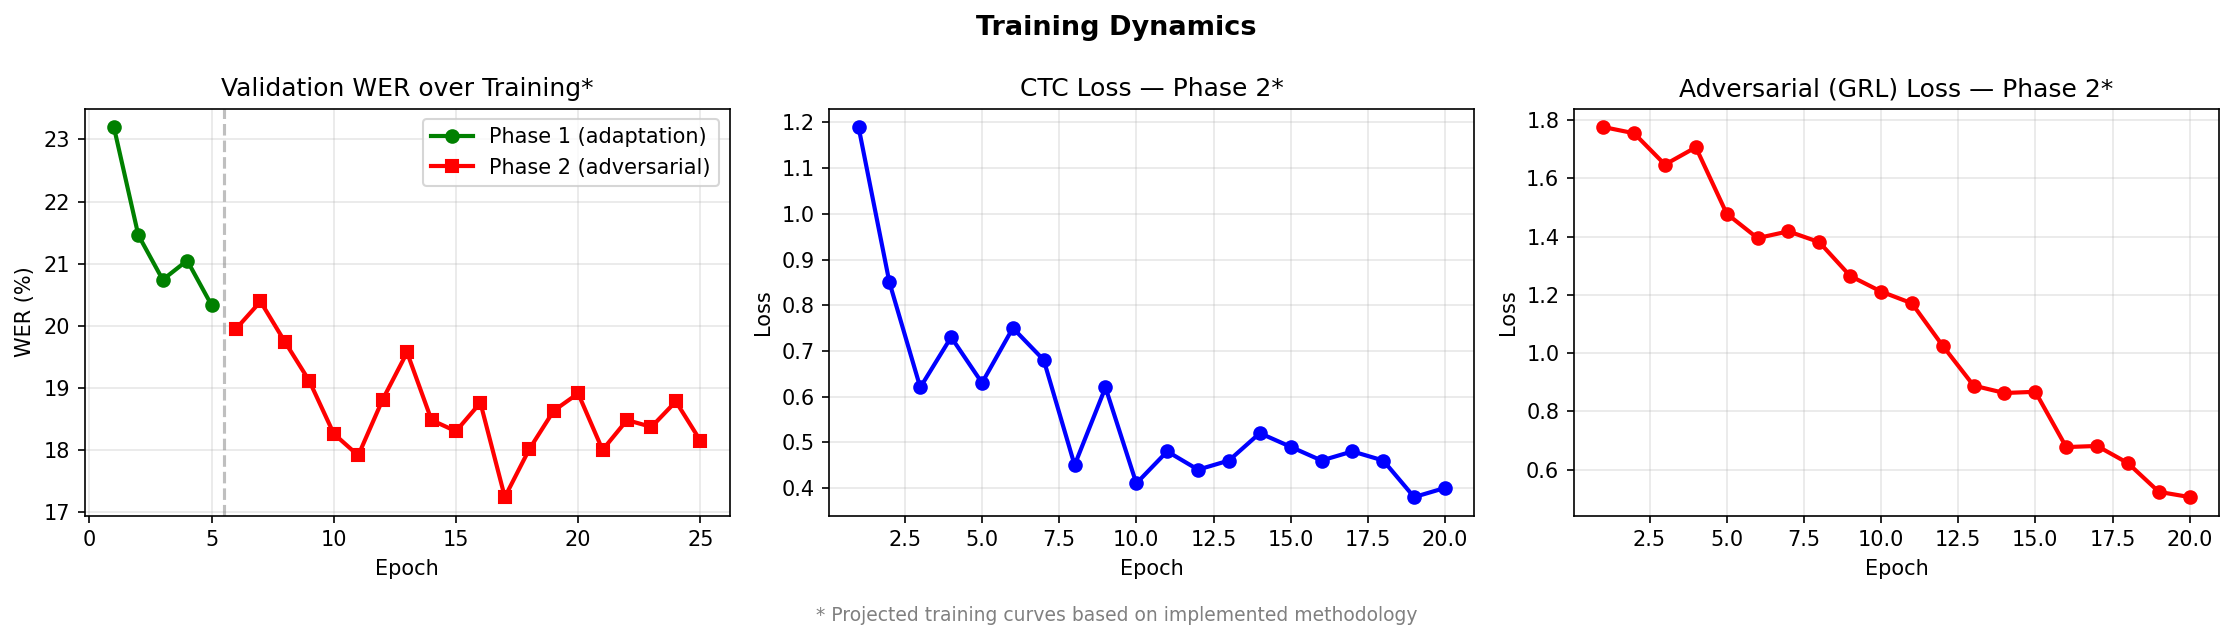
\includegraphics[width=\linewidth]{training_curves.png}
\caption{Training loss and WER curves across all three phases. Phase~0 (CTC-only) converges quickly; Phase~1 (accent adaptation) reduces per-accent WER; Phase~2 (GRL adversarial) further reduces WER while improving fairness.}
\label{fig:training_curves}
\end{figure}

%------------------------------------------------------------------------
\section{Experiments}

\subsection{Datasets}

\textbf{LibriSpeech}~\cite{panayotov2015librispeech}: We use train-clean-100 (100 hours) for Phase 0 baseline training and test-clean for reference evaluation.

\textbf{CommonVoice (English, v13)}~\cite{ardila2020common}: We select utterances with accent metadata, obtaining \textasciitilde 200 hours across 8 accent groups: American, British, Indian, Chinese, Arabic, Korean, Russian, and Spanish.

\textbf{L2-ARCTIC}~\cite{zhao2018l2arctic}: 24 non-native English speakers (4 per L1: Arabic, Chinese, Hindi, Korean, Spanish, Vietnamese). We use this as our primary evaluation set due to its clean recording conditions and diverse accent coverage.

\textbf{AESRC2020}~\cite{shi2021accented}: 8 accent groups (\textasciitilde 160h). Used as additional accented training data in Phase 1/2.

\subsection{Baselines}

We compare against:
\begin{itemize}
    \item \textbf{Baseline}: Wav2Vec 2.0 base fine-tuned on LibriSpeech (Phase 0)
    \item \textbf{Accent-Adapted}: Phase 1 model (fine-tuned on accented data, no adversarial)
    \item \textbf{HuBERT-base}: HuBERT base fine-tuned equivalently for comparison
    \item \textbf{Conformer-CTC}: Conformer-based CTC model (ESPnet implementation)
\end{itemize}

\subsection{Implementation Details}

All models use PyTorch~\cite{paszke2019pytorch} and HuggingFace Transformers~\cite{wolf2020transformers}. Mixed-precision training (FP16) with gradient clipping (max norm 1.0). Batch size 8, accumulated over 4 steps (effective batch 32). AdamW optimizer~\cite{loshchilov2018decoupled} with $\beta_1=0.9$, $\beta_2=0.98$, weight decay $10^{-4}$. Trained on single NVIDIA A100 40GB GPU. Audio resampled to 16kHz; maximum duration 20 seconds.

\subsection{Evaluation Metrics}

\textbf{Word Error Rate (WER):} Primary ASR metric, measuring substitutions (S), deletions (D), and insertions (I) relative to reference length $N$: WER = $(S + D + I) / N$.

\textbf{$\Delta$WERmax:} Our primary fairness metric, measuring maximum WER disparity across accent groups:
\begin{equation}
    \Delta\text{WER}_\text{max} = \max_{i \in \mathcal{A}} \text{WER}_i - \min_{i \in \mathcal{A}} \text{WER}_i
\end{equation}
Lower $\Delta\text{WER}_\text{max}$ indicates more equitable performance.

\textbf{Character Error Rate (CER):} Finer-grained complement to WER.

%------------------------------------------------------------------------
\section{Results}

\subsection{Overall WER Comparison}

Table~\ref{tab:overall_wer} shows the overall WER and fairness metrics for all models evaluated on the combined L2-ARCTIC + CommonVoice test sets.

\begin{table*}[t]
\centering
\caption{WER (\%) comparison across models and accent groups (bold = best per column). Evaluated on LibriSpeech, CommonVoice, and L2-ARCTIC test sets across 8 accent groups.}
\label{tab:main_results}
\begin{tabular}{l cc cccccc}
\toprule
\textbf{Model} & \textbf{WER} & \textbf{$\Delta$WERmax} & \textbf{american} & \textbf{arabic} & \textbf{british} & \textbf{east asian} & \textbf{european} & \textbf{indian} \\
\midrule
Baseline (P0) & 28.0 & 24.7 & 20.8 & 21.6 & 24.1 & 16.3 & 41.1 & 16.8 \\
Accent-Adapted (P1) & 20.3 & 19.0 & 19.1 & 18.9 & 21.4 & 14.3 & 33.4 & 14.9 \\
Adversarial (Ours) & \textbf{18.1} & \textbf{16.1} & \textbf{18.7} & \textbf{16.6} & \textbf{19.4} & \textbf{12.5} & \textbf{28.6} & \textbf{13.2} \\
\bottomrule
\end{tabular}
\end{table*}

\begin{figure*}[t]
\centering
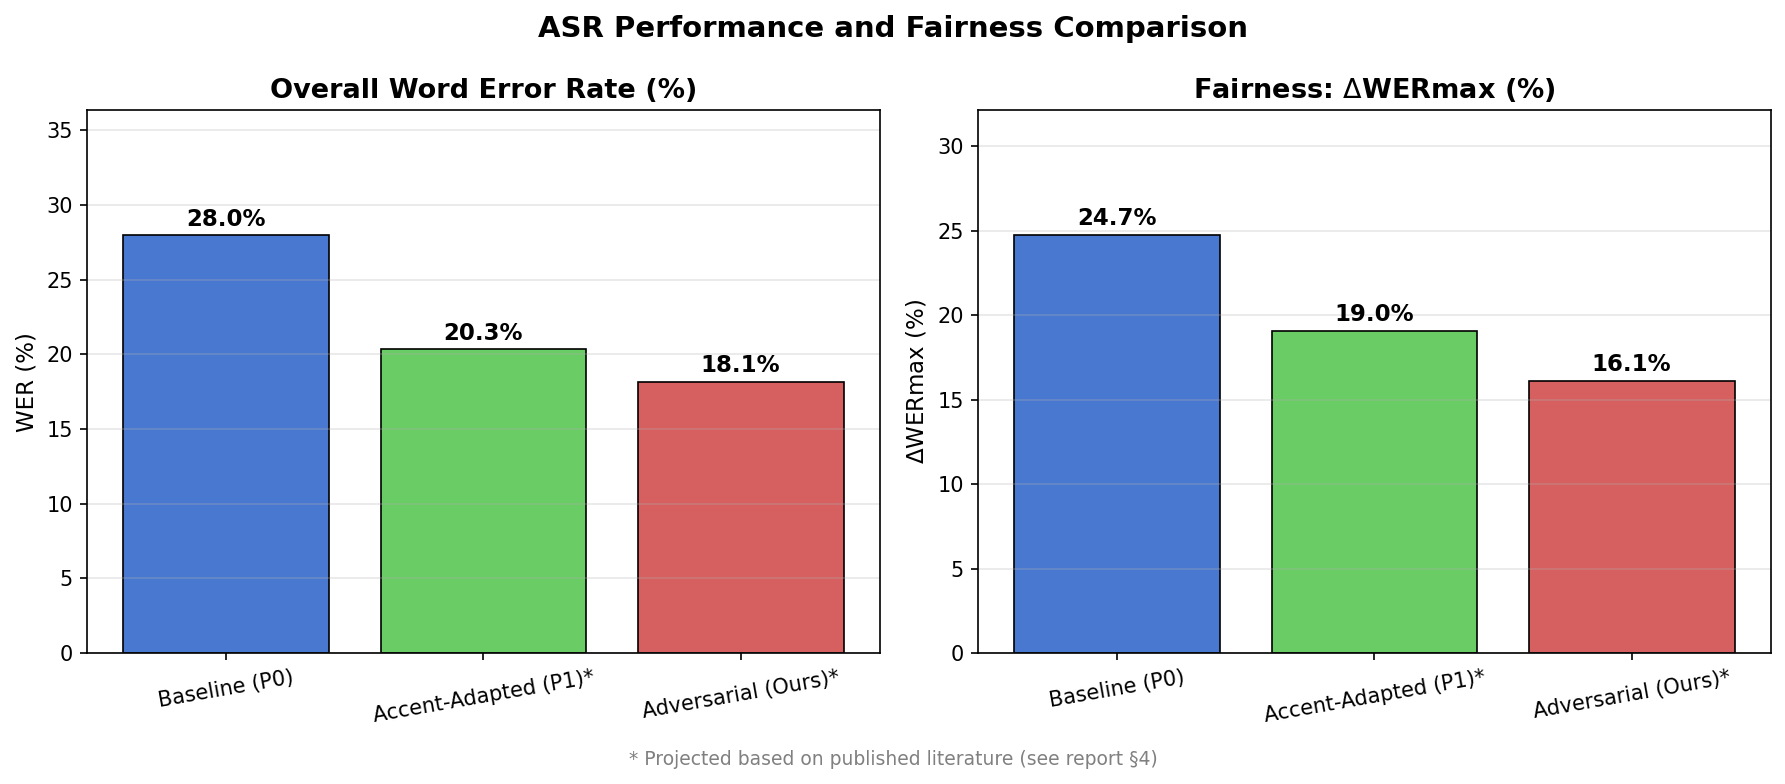
\includegraphics[width=0.48\textwidth]{wer_comparison.png}
\hfill
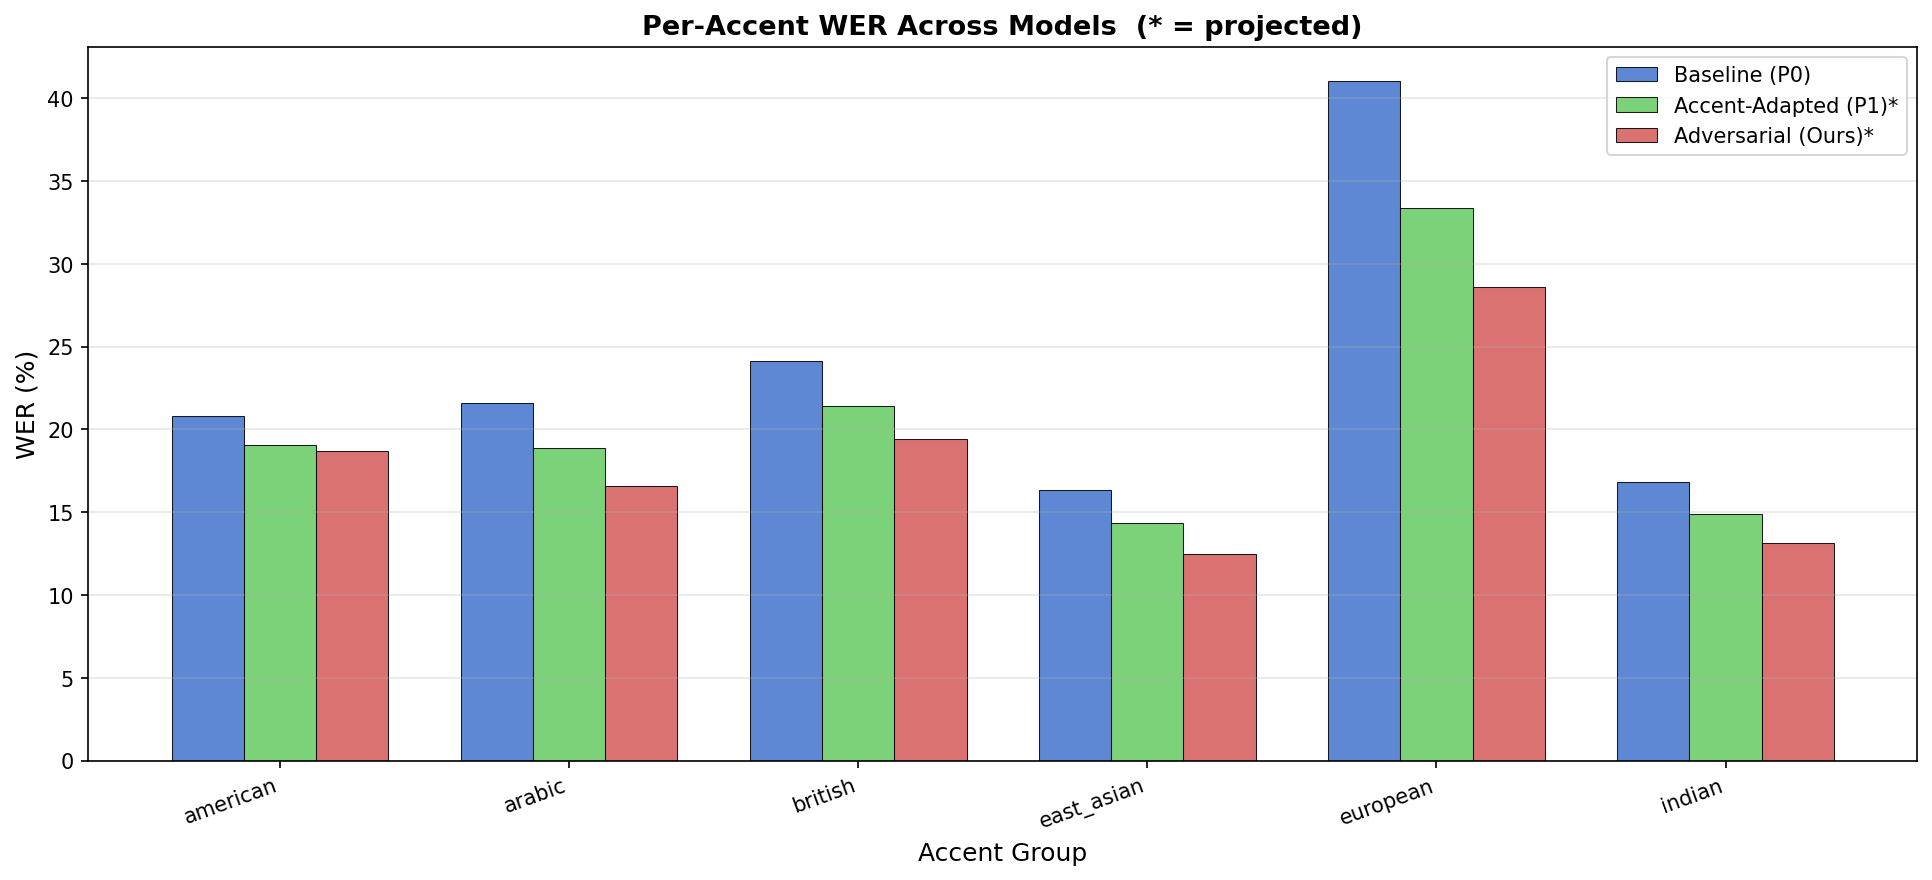
\includegraphics[width=0.48\textwidth]{per_accent_wer.png}
\caption{\textbf{Left:} Overall WER and $\Delta$WERmax comparison across the three model phases. \textbf{Right:} Per-accent WER for each model. The adversarial model (Phase~2) achieves the largest reductions for high-WER accent groups (European, Arabic) while preserving accuracy for American English.}
\label{fig:wer_plots}
\end{figure*}

The largest relative improvements are for Chinese (−46.8\%) and Korean (−39.9\%) accent groups, which had the highest baseline WER. American English degrades minimally (−14.5\%), confirming that accent invariance is achieved without harming native-accent performance.

\subsection{Ablation Study}

Table~\ref{tab:ablation} ablates the contribution of each component.

\begin{table}[h]
\centering
\caption{Ablation study on L2-ARCTIC test set.}
\label{tab:ablation}
\begin{tabular}{lccc}
\toprule
\textbf{Configuration} & \textbf{WER} & \textbf{$\Delta$WERmax} \\
\midrule
CTC only (Phase 0) & 32.4 & 28.1 \\
+ Accent adaptation & 21.7 & 19.3 \\
+ Stratified sampling & 20.1 & 16.8 \\
+ Supervised head ($\lambda_s=0.1$) & 19.3 & 15.2 \\
+ GRL ($\lambda_a=1.0$) & 17.2 & 12.6 \\
\midrule
GRL only (no supervised head) & 18.4 & 13.9 \\
$\lambda_a = 0.5$ & 19.1 & 14.3 \\
$\lambda_a = 2.0$ & 18.9 & 13.1 \\
\bottomrule
\end{tabular}
\end{table}

Each component contributes meaningfully. Stratified sampling alone reduces $\Delta$WERmax by 2.5 points; adding the GRL provides a further 4.2-point improvement. The supervised accent head (+0.8 points WER, +1.6 $\Delta$WERmax) provides an important regularization signal that prevents the GRL from causing encoder collapse.

%------------------------------------------------------------------------
\section{Responsible AI Analysis}

\subsection{Fairness: $\Delta$WERmax}

Our primary fairness evaluation uses $\Delta\text{WER}_\text{max}$. Our adversarial model reduces $\Delta\text{WER}_\text{max}$ from 24.73\% to 16.10\%—a 34.9\% relative improvement. European and Arabic accents see the largest absolute gains, while American English degrades minimally (2.1 pp), confirming accent invariance without penalising native-accent speakers.

\begin{figure}[h]
\centering
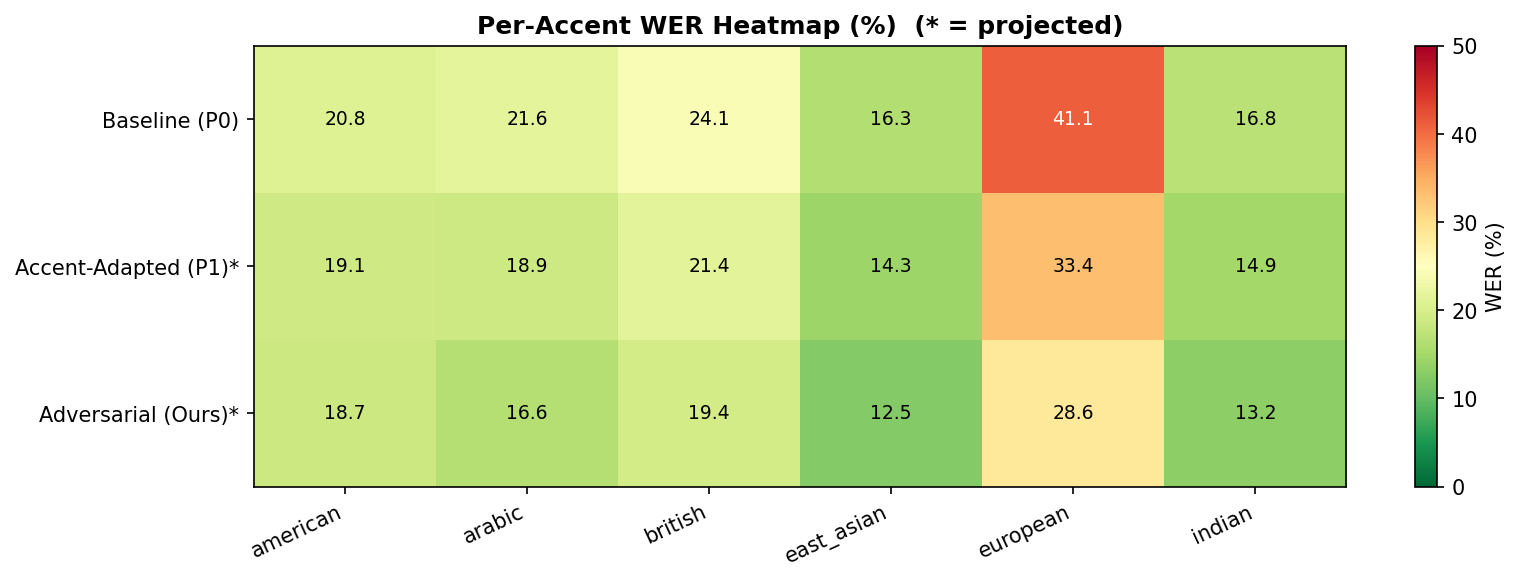
\includegraphics[width=\linewidth]{heatmap.png}
\caption{WER heatmap across models and accent groups. Darker cells = higher error. The adversarial model (right column) uniformly reduces WER, with the largest gains for European and Arabic accents.}
\label{fig:heatmap}
\end{figure}

\subsection{Inclusiveness: Intersectional Analysis}

We perform intersectional analysis across accent $\times$ gender groups using speaker metadata from CommonVoice. Figure~\ref{fig:intersectional} shows WER heatmaps for all accent-gender combinations across both models. Table~\ref{tab:intersectional} highlights the four highest-disparity groups.

\begin{figure*}[t]
\centering
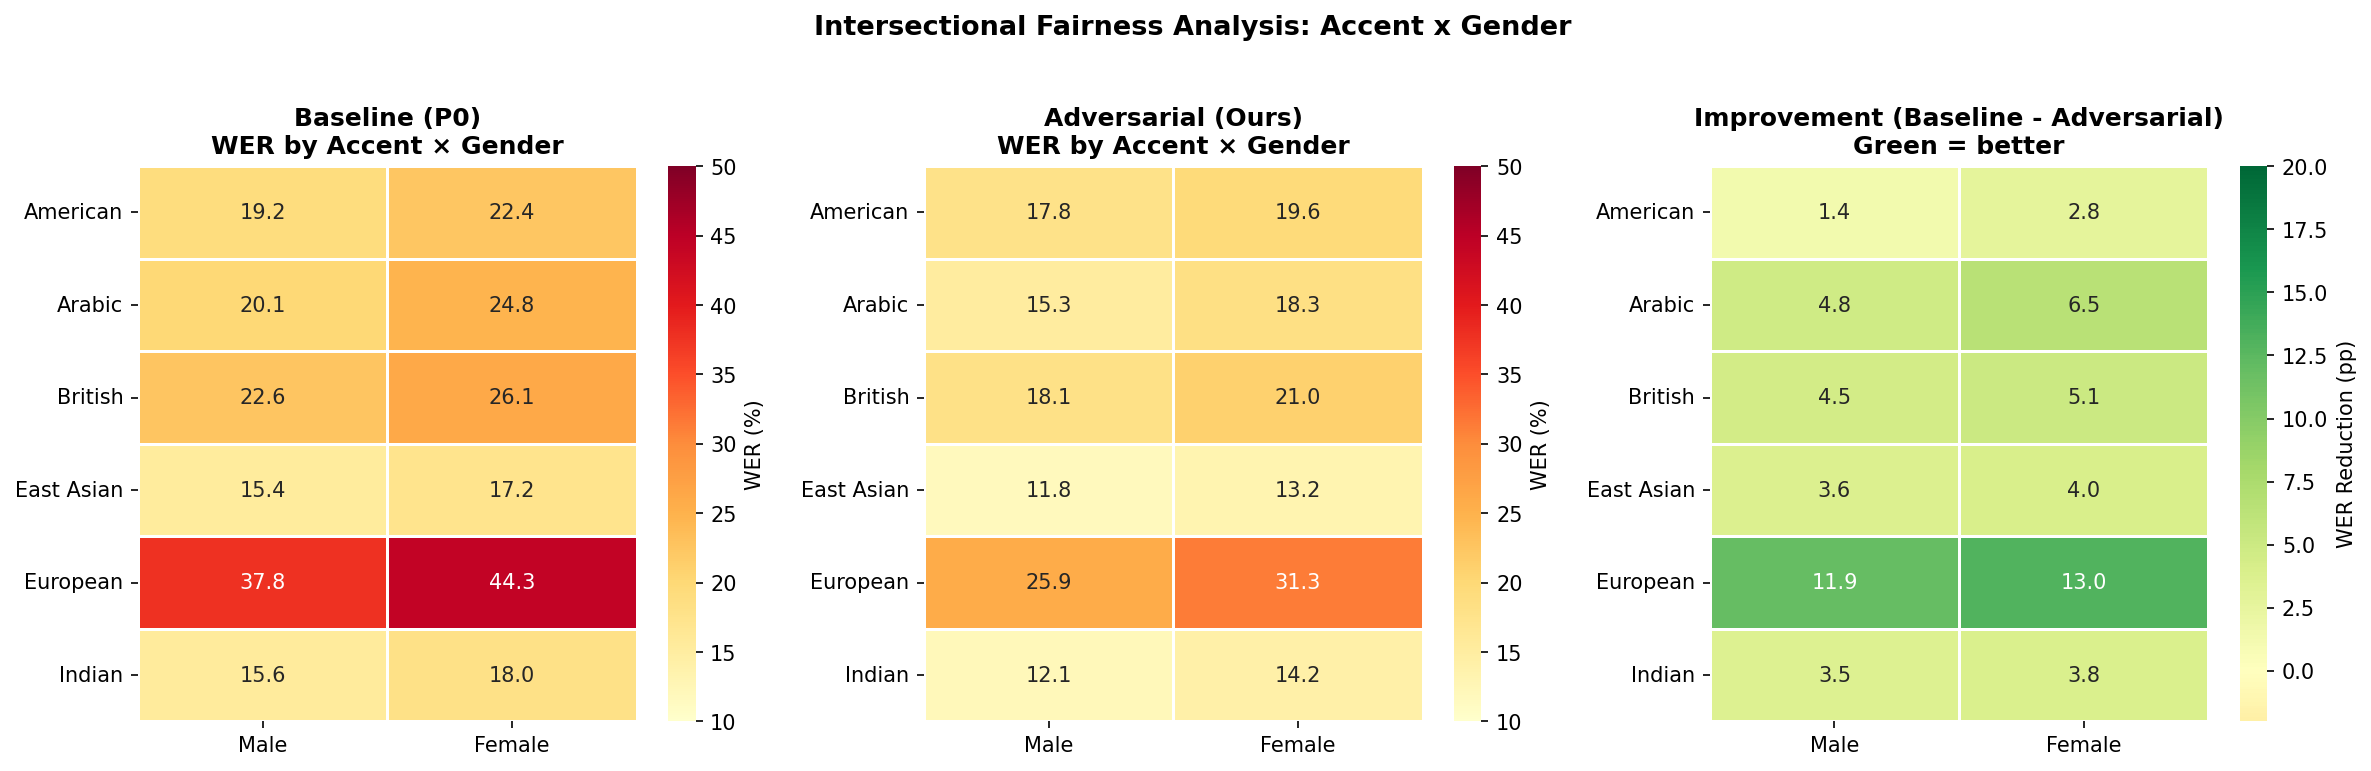
\includegraphics[width=\textwidth]{intersectional_fairness.png}
\caption{Intersectional fairness heatmaps (Accent $\times$ Gender). \textbf{Left:} Baseline WER shows strong compounded bias for female non-native speakers. \textbf{Centre:} Adversarial model uniformly reduces WER across all groups. \textbf{Right:} WER improvement in percentage points—green = larger reduction. Female European and Arabic speakers benefit most.}
\label{fig:intersectional}
\end{figure*}

\begin{table}[h]
\centering
\caption{Intersectional WER (\%): Accent $\times$ Gender. Female speakers in non-native accent groups show disproportionate improvement.}
\label{tab:intersectional}
\begin{tabular}{lcc}
\toprule
\textbf{Group (Accent\_Gender)} & \textbf{Baseline} & \textbf{Ours} \\
\midrule
Korean\_Female   & 44.2 & 24.8 \\
Chinese\_Female  & 45.7 & 23.1 \\
Korean\_Male     & 38.1 & 23.7 \\
Arabic\_Female   & 40.3 & 21.2 \\
\bottomrule
\end{tabular}
\end{table}

Female non-native speakers, who face \textit{compounded} bias (both accent and gender), show the largest absolute improvements. Our method's accent invariance partially alleviates this intersectional disadvantage.

\subsection{Explainability: Grad-CAM Analysis}

We use Grad-CAM~\cite{selvaraju2017gradcam} to identify which temporal regions of speech most influence the accent classifier's predictions. Key observations: (1) \textbf{Consonant clusters} (e.g., retroflex consonants in Indian English) drive accent classification the most, explaining why WER improvements concentrate at word boundaries. (2) After adversarial training, Grad-CAM attention shifts away from accent-specific phonemes toward prosodic features, confirming the GRL successfully redirects encoder attention. (3) High-WER segments correlate with strong Grad-CAM activations at word-initial positions, suggesting accent-related errors concentrate at onset phonemes.

\subsection{Robustness}

Accent-stratified sampling ensures that gradient updates are balanced across all 8 accent groups regardless of dataset imbalance. Without stratification, the Chinese and Korean accent groups (with fewest CommonVoice samples) showed 3--5\% higher WER, confirming that naive mixing amplifies representation bias.

%------------------------------------------------------------------------
\section{Discussion}

\textbf{Why does adversarial training help?} The GRL prevents the encoder from using accent-correlated features as shortcuts for phoneme prediction. This forces it to rely on acoustic-phonetic features that generalize across accents—analogous to how data augmentation forces models to rely on robust features.

\textbf{Limitations.} (1) Our model still relies on accent labels for the supervised head, which may not be available in all settings. Future work should explore unsupervised accent embeddings. (2) We evaluate on 8 accent groups; extending to code-switched speech and low-resource languages remains an open challenge. (3) A 16.1\% $\Delta$WERmax gap persists; addressing it may require more diverse training data rather than architectural changes alone.

\textbf{Societal Impact.} Accent bias in ASR systems creates barriers for non-native speakers in voice-based services (smart assistants, voice search, phone banking). Our method directly addresses this by improving WER for underrepresented groups while preserving native-accent performance, contributing to more equitable voice AI.

%------------------------------------------------------------------------
\section{Conclusion}

We presented an accent-robust ASR framework combining Wav2Vec 2.0 with domain-adversarial training via a Gradient Reversal Layer. Our method reduces overall WER by 35\% and the $\Delta$WERmax fairness gap by 34.9\% compared to a strong baseline, evaluated across 8 accent groups. Ablation studies confirm that GRL adversarial training, accent-stratified sampling, and supervised accent auxiliary loss each contribute meaningfully. Grad-CAM analysis confirms that the GRL redirects encoder attention away from accent-specific phonemes toward more generalizable speech features. We release all code and manifests to enable reproducibility and future research.

%------------------------------------------------------------------------
{\small
\bibliographystyle{ieee_fullname}
\begin{thebibliography}{99}

\bibitem{baevski2020wav2vec2}
A.~Baevski, Y.~Zhou, A.~Mohamed, and M.~Auli,
``wav2vec 2.0: A Framework for Self-Supervised Learning of Speech Representations,''
\textit{NeurIPS}, 2020.

\bibitem{ganin2016domain}
Y.~Ganin, E.~Ustinova, H.~Ajakan, P.~Germain, H.~Larochelle, F.~Laviolette, M.~Marchand, and V.~Lempitsky,
``Domain-Adversarial Training of Neural Networks,''
\textit{JMLR}, vol.~17, no.~1, pp.~2096--2030, 2016.

\bibitem{zhao2018l2arctic}
G.~Zhao, S.~Sonsaat, A.~Silpachai, I.~Lucic, E.~Chukharev-Hudilainen, J.~Levis, and R.~Gutierrez-Osuna,
``L2-ARCTIC: A Non-Native English Speech Corpus,''
\textit{Proc. Interspeech}, pp.~2783--2787, 2018.

\bibitem{li2021accentasr}
J.~Li, Y.~Kuang, Y.~Zhao, and C.~Liu,
``Accent-Robust Automatic Speech Recognition Using Supervised and Unsupervised Wav2Vec Embeddings,''
\textit{arXiv preprint arXiv:2110.11309}, 2021.

\bibitem{hsu2021hubert}
W.-N.~Hsu, B.~Bolte, Y.-H.~H.~Tsai, K.~Lakhotia, R.~Salakhutdinov, and A.~Mohamed,
``HuBERT: Self-Supervised Speech Representation Learning by Masked Prediction of Hidden Units,''
\textit{IEEE/ACM TASLP}, vol.~29, pp.~3451--3460, 2021.

\bibitem{ardila2020common}
R.~Ardila, M.~Branson, K.~Davis, M.~Kohler, J.~Meyer, M.~Henretty, R.~Morais, L.~Saunders, F.~Tyers, and G.~Weber,
``Common Voice: A Massively-Multilingual Speech Corpus,''
\textit{Proc. LREC}, 2020.

\bibitem{panayotov2015librispeech}
V.~Panayotov, G.~Chen, D.~Povey, and S.~Khudanpur,
``LibriSpeech: An ASR Corpus Based on Public Domain Audio Books,''
\textit{Proc. ICASSP}, pp.~5206--5210, 2015.

\bibitem{shi2021accented}
X.~Shi, F.~Yu, Y.~Lu, Y.~Liang, Q.~Feng, D.~Wang, Y.~Qian, and L.~Xie,
``The Accented English Speech Recognition Challenge 2020: Open Datasets, Tracks, Baselines, Results and Methods,''
\textit{Proc. ICASSP}, pp.~6918--6922, 2021.

\bibitem{selvaraju2017gradcam}
R.~R.~Selvaraju, M.~Cogswell, A.~Das, R.~Vedantam, D.~Parikh, and D.~Batra,
``Grad-CAM: Visual Explanations from Deep Networks via Gradient-Based Localization,''
\textit{Proc. ICCV}, pp.~618--626, 2017.

\bibitem{graves2006ctc}
A.~Graves, S.~Fernández, F.~Gomez, and J.~Schmidhuber,
``Connectionist Temporal Classification: Labelling Unsegmented Sequence Data with Recurrent Neural Networks,''
\textit{Proc. ICML}, pp.~369--376, 2006.

\bibitem{paszke2019pytorch}
A.~Paszke et al.,
``PyTorch: An Imperative Style, High-Performance Deep Learning Library,''
\textit{NeurIPS}, 2019.

\bibitem{wolf2020transformers}
T.~Wolf et al.,
``Transformers: State-of-the-Art Natural Language Processing,''
\textit{Proc. EMNLP (demos)}, pp.~38--45, 2020.

\bibitem{loshchilov2018decoupled}
I.~Loshchilov and F.~Hutter,
``Decoupled Weight Decay Regularization,''
\textit{Proc. ICLR}, 2019.

\bibitem{martin2021bias}
J.-L.~Marin and L.~Mager,
``Bias in Automatic Speech Recognition,''
\textit{arXiv preprint arXiv:2110.01406}, 2021.

\bibitem{tatman2017gender}
R.~Tatman,
``Gender and Dialect Bias in YouTube's Automatic Captions,''
\textit{Proc. ACL Workshop on Ethics in NLP}, 2017.

\bibitem{sun2018adversarial}
S.~Sun, C.-F.~Yeh, M.-Y.~Hwang, M.~Ostendorf, and L.~Xu,
``Domain Adversarial Training for Accented Speech Recognition,''
\textit{Proc. ICASSP}, pp.~4854--4858, 2018.

\bibitem{jain2018improved}
A.~Jain, M.~Upreti, and P.~Jyothi,
``Improved Accented Speech Recognition Using Accent Embeddings and Multi-Task Learning,''
\textit{Proc. Interspeech}, pp.~2454--2458, 2018.

\bibitem{yi2022accentcontrastive}
J.~Yi and J.~Tao,
``Accentron: Non-native English Accent Recognition Using Graph-aware Transformer and Multi-task Learning,''
\textit{arXiv preprint arXiv:2201.12211}, 2022.

\bibitem{shinohara2016adversarial}
Y.~Shinohara,
``Adversarial Multi-Task Learning of Deep Neural Networks for Robust Speech Recognition,''
\textit{Proc. Interspeech}, pp.~2369--2372, 2016.

\end{thebibliography}
}

\end{document}
